\usetikzlibrary{positioning, shapes.symbols, shapes.geometric, arrows.meta, calc, fit, backgrounds, shadows, matrix}

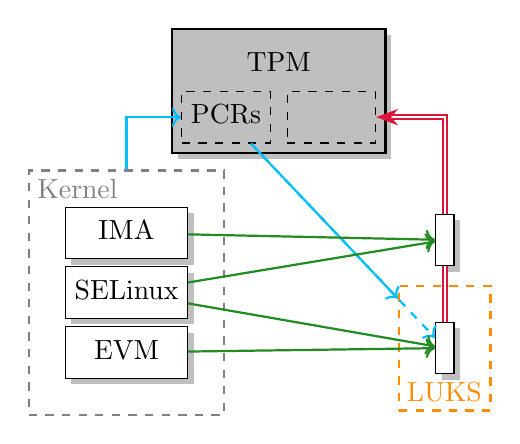
\begin{tikzpicture}[
    required_by/.style={->,thick,DeepSkyBlue},
    protects/.style={->,thick,ForestGreen},
    box/.style={drop shadow, fill=white}
]

\node (TPM) at (0,0) {TPM\strut};
\node [below left=0 and 0.1 of TPM.south, anchor=north east, draw, dashed] (PCRs) {PCRs\strut};
\node [below right=0 and 0.1 of TPM.south, anchor=north west, text width=width("PCRs"), align=center, draw, dashed] (Key) {\pk\strut};
\begin{scope}[on background layer]
    \node[draw, box, fill=lightgray, solid, thick, fit=(TPM) (PCRs) (Key)] (TPMbg) {};
\end{scope}

\matrix (m) [
    matrix of nodes,
    nodes={draw, box, text width=width("SELinux"), align=flush center},
    row sep=.25em,
] at (-5.5em,-8.25em) {
    |(IMA)| IMA\strut \\
    |(SELinux)| SELinux\strut \\
    |(EVM)| EVM\strut \\
  };
\node [draw, gray, dashed, thick, inner sep=.95em, fit=(m),
        label={[gray, anchor=north west]north west:Kernel}] (Kernel) {};

\node [box] (WCP) at (6em,-10.25em) [draw] {\wcp\strut};
\node [draw, DarkOrange, dashed, thick, fit=(WCP), inner sep=1.3em,
        label={[DarkOrange, anchor=south east]south east:LUKS}] (LUKS) {};
\node [box, above=2em of WCP] (tpm_sign) [draw] {\tpmsign\strut};

\draw[required_by] (Kernel) |- (PCRs);
\draw[required_by, dashed] (PCRs) -- (WCP);
\draw[required_by] (PCRs) -- (LUKS);

\draw[protects] (EVM) -- (WCP);
\draw[protects] (SELinux) -- (WCP);
\draw[protects] (SELinux) -- (tpm_sign);
\draw[protects] (IMA) -- (tpm_sign);


\draw[-, thick, double, Crimson] (WCP) -- (tpm_sign);
\draw[-{Stealth}, thick, double, Crimson] (tpm_sign) |- (Key);

\end{tikzpicture}